\paragraph{Not fixed cells imaging as corrupted input}
    \begin{figure}[H]
        \begin{center}
            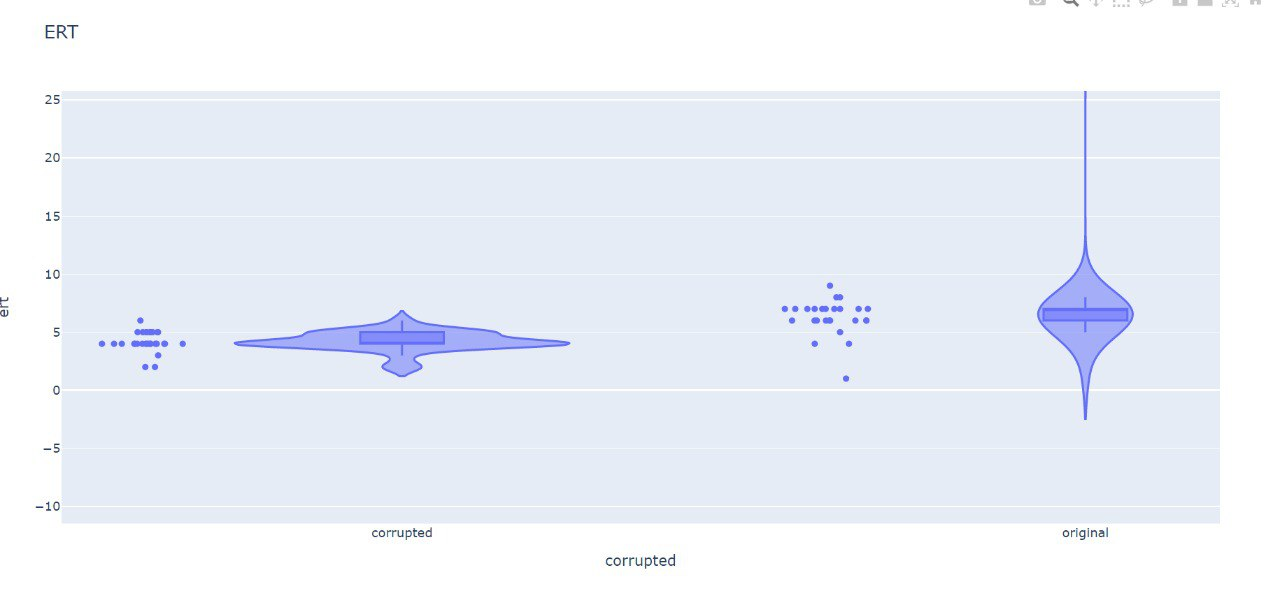
\includegraphics[width=0.5\linewidth]{bilder/drift-detection/online-fixed-vs-not-fixed.jpg}
            \caption{Online drift detection of not fixated cells}\label{fig:online-drift-not-fixed}
        \end{center}
    \end{figure}

    Scores of 0.91 however the threshold is 6, not corrupted data (fixed cells) mostly ert of 7 whereas corrupted data (not fixed cells) have an ert of 4. The threshold is therefore 6.

\paragraph{Real-world examples of corruptions}
